\section{CONCEITOS GERAIS E REVISÃO DA LITERATURA}

Nesta seção, apresentam-se os conceitos teóricos fundamentais que alicerçam este estudo, fornecendo a base conceitual necessária para a compreensão das análises subsequentes. Inicialmente, exploram-se os fundamentos teóricos que norteiam a pesquisa, abordando a Engenharia de Requisitos e o Teste de \textit{software}. Por fim, expõe-se uma revisão da literatura, destacando trabalhos correlatos voltados à identificação e mitigação de DTs.

\subsection{Engenharia de Requisitos e Teste de Software}
\label{sec:engenharia_requisitos_teste_software}

Define-se a engenharia de software como a ``aplicação sistemática de métodos, conhecimentos e experiências científicas e tecnológicas no design, implementação, teste e documentação de software''~\cite[p. 424, tradução nossa]{27}. Historicamente, essa disciplina emergiu durante o período referenciado como crise do software, em 1968~\cite{28}. Desde então, diversas metodologias foram propostas em seu escopo com o objetivo de sistematizar e dar suporte ao desenvolvimento de projetos de software.

Dentre essas metodologias, as práticas voltadas para a engenharia de requisitos destacam-se como fundamentais, alinhando-se diretamente à problemática da defasagem documental levantada na introdução deste trabalho. Nesse contexto, para a representação formal do comportamento esperado e das funcionalidades que o sistema deve contemplar, os casos de uso (CdUs)~\cite{2} consolidam-se como uma das abordagens mais adotadas. A ampla aceitação desse método deve-se ao fato de consistir na descrição de ``uma história de como um usuário final interage com o sistema dentro de um conjunto de circunstâncias específicas'' (Pressman e Maxim~\cite[p. 114, tradução nossa]{24}). Essa particularidade promove o alinhamento entre a especificação técnica e a visão prática do \textit{stakeholder} --- termo que designa qualquer parte interessada no produto, abrangendo desde os patrocinadores até os usuários finais. Estruturalmente, tais descrições podem ser documentadas em formato de texto corrido (como histórias de usuário), em etapas sequenciais ou por meio de diagramas~\cite{24}. Por esse motivo, a modelagem de casos de uso configura-se como um processo mais intuitivo e condizente com a realidade do projeto, desde que os objetivos e as expectativas dos envolvidos tenham sido previamente compreendidos.

Contudo, apenas definir o comportamento esperado de um sistema não é suficiente; torna-se imperativo garantir a exatidão dessa definição e assegurar que o software seja implementado em estrita conformidade com essa especificação. Por essa razão, a execução de testes ao longo de todas as fases de desenvolvimento é considerada uma atividade inerente e indispensável em projetos de software~\cite{6,7}. Essa prática viabiliza duas frentes de garantia de qualidade fundamentais: a validação --- cujo propósito é confirmar se o produto correto está sendo construído para atender às necessidades do usuário --- e a verificação --- destinada a avaliar se o produto está sendo construído corretamente, de acordo com os seus requisitos~\cite{21}. Nesse sentido, faz-se necessária a discussão das principais abordagens de teste voltadas para a verificação do software, com o intuito de delinear a inserção dessas práticas no escopo prático deste trabalho.

Pressman e Maxim~\cite{24} estruturam as etapas de teste conforme ilustrado na Figura~\ref{fig:etapas_teste}. Inicialmente, a condução dos testes de unidade tem como foco a verificação individual de cada componente, com o propósito de assegurar o seu funcionamento isolado e atestar a corretude das menores estruturas do sistema, como funções e classes. Em seguida, durante a fase de testes de integração, esses elementos previamente validados são agrupados em conformidade com a arquitetura do software, visando à identificação de falhas nas interfaces de comunicação entre eles. Adicionalmente, essa etapa abrange a verificação da interoperabilidade do sistema com dependências externas, a exemplo de bancos de dados e Interfaces de Programação de Aplicações (APIs) de terceiros. Por fim, por meio dos testes de alta ordem, também conhecidos como testes de sistema, o software é avaliado em sua totalidade. Nesse estágio, atesta-se tanto o atendimento integral de suas funcionalidades quanto a satisfação dos requisitos de desempenho preestabelecidos.

\begin{figure}[t]
    \centering
    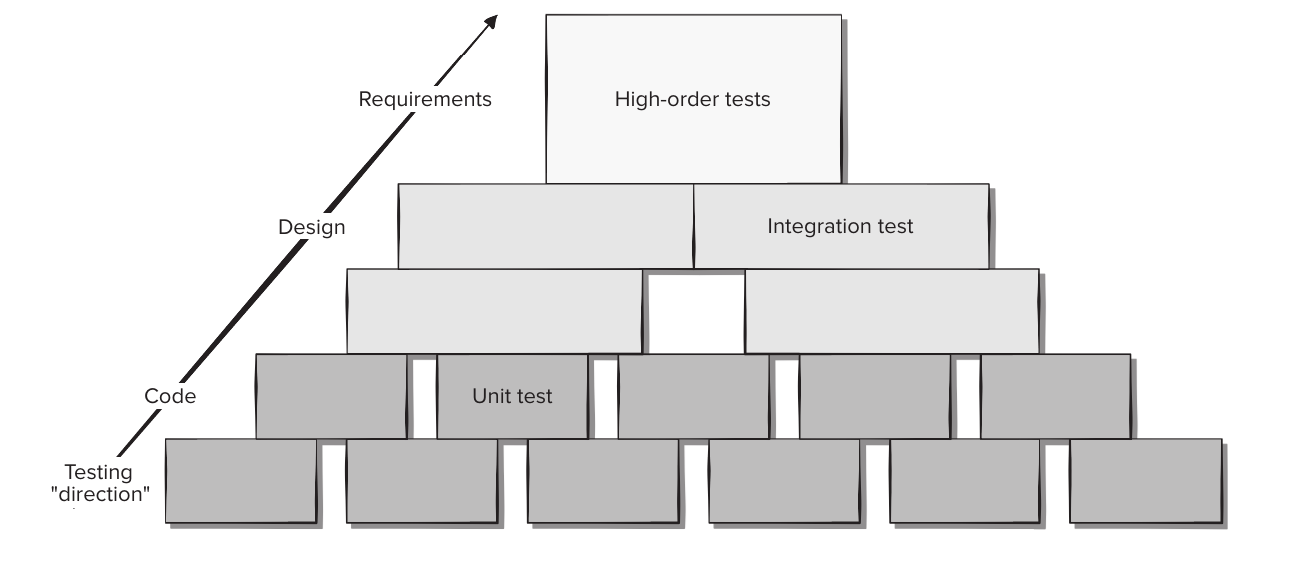
\includegraphics[height=6.2cm]{imagens/etapas_teste.png}
    \caption{Etapas de teste de software}

    \vspace{3pt}
    {\small\textbf{Fonte}: Pressman e Maxin~\cite[p. 376]{24}}
    \label{fig:etapas_teste}
\end{figure}

Adicionalmente, o escopo da engenharia de software abrange práticas ágeis focadas no alinhamento entre a especificação de requisitos e o teste do sistema. Dentre elas, destaca-se o \textit{Behaviour-Driven Development} (BDD), introduzido por North~\cite{26}. Nessa abordagem, as funcionalidades são concebidas como comportamentos do software, sendo especificadas por meio de uma linguagem natural fundamentada em palavras-chave que atuam como conectivos lógicos para as ações. Desse modo, o BDD configura-se como um mecanismo de especificação análogo aos casos de uso, diferenciando-se, contudo, por adotar um formato mais conciso e voltado à legibilidade mútua entre as partes técnicas e as ferramentas de automação para testes de software. Para fins de ilustração, apresenta-se no Quadro \ref{qua:historia_usuario} o exemplo de uma história de usuário.

Essa mesma história de usuário poderia ser especificada por meio de um caso de uso, conforme ilustrado no Quadro~\ref{qua:exemplo_caso_de_uso}. Nessa representação, delineiam-se o fluxo principal e o fluxo de exceção. No primeiro, são descritas as condições normais de operação para a concretização do objetivo, enquanto no segundo, estabelece-se o comportamento esperado do sistema diante de falhas ou impedimentos. Sob a ótica do BDD, essa funcionalidade seria estruturada conforme os cenários apresentados no Quadro \ref{qua:exemplo_bdd}, nos quais o primeiro cenário é análogo ao fluxo principal e o segundo, ao fluxo de exceção.



Uma das principais vantagens do BDD reside no emprego da linguagem natural para a descrição comportamental. Conforme demonstrado no exemplo anterior, essa especificação é prontamente compreendida tanto por stakeholders quanto por desenvolvedores, o que promove a comunicação e a transparência entre as partes envolvidas. Adicionalmente, a estruturação em cenários permite identificar, de maneira objetiva, as variações nas respostas do sistema diante do atendimento, ou não, de diferentes critérios. Ao reanalisar o cenário supracitado, constata-se que a alteração de um único pré-requisito (a disponibilidade de crédito) reconfigura o fluxo de execução. Essa acessibilidade na leitura atua em contraponto à granularidade técnica intrínseca aos casos de uso. Embora a interpretação deste último artefato demande maior familiaridade técnica, o seu nível de detalhamento delineia com precisão a lógica interna do software, conferindo um suporte mais diretivo à fase de implementação quando comparado ao BDD.

\begin{quadro}[t]
    \centering
    
    \caption{Exemplo de estruturação de uma História de Usuário para a funcionalidade de saque}
    \label{qua:historia_usuario}
    
    \fcolorbox{black}{backcolour}{% 
        \begin{minipage}{0.9\textwidth}\small%
            \vspace{3pt}%
            \normalsize{\textbf{Título:} Sacar dinheiro de um caixa rápido}\vspace{5pt}\\
                \hspace*{1.25cm}\textbf{Como} um cliente,\\
                \hspace*{1.25cm}\textbf{quero} resgatar dinheiro através de um caixa rápido\\
                \hspace*{1.25cm}\textbf{para} que eu não tenha que esperar em uma fila no banco.
    \end{minipage}
    }
    
    \vspace{5pt}
    \hspace*{0.75cm}\raggedright{\small \textbf{Fonte:} Elaborado pelo autor.}
\end{quadro}

\begin{quadro}[h!]
    \centering
    \caption{Exemplo de especificação textual de um Caso de Uso para a funcionalidade de saque}
    \label{qua:exemplo_caso_de_uso}
    
    \fcolorbox{black}{backcolour}{% 
        \begin{minipage}{0.9\textwidth}\small%
            \vspace{3pt}%
            \noindent\textbf{\normalsize CdU1 - Efetuar saque em caixa eletrônico}\vspace{5pt}\\
            \textbf{Agente:} Cliente\\
            \textbf{Pré-Condições:}
            \begin{itemize}[topsep=0pt]
                \itemsep0em
                \item O terminal do caixa eletrônico deve estar operante, conectado à rede bancária e abastecido com cédulas. 
                \item O cliente deve possuir um cartão válido e conhecer sua respectiva credencial de acesso (senha).
            \end{itemize}
            \textbf{Fluxo Principal:}
            \begin{enumerate}[topsep=0pt]
                \itemsep0em
                \item O cliente insere o cartão no terminal do caixa eletrônico.
                \item O sistema faz a leitura do cartão e solicita e apresenta o menu de operações.
                \item O cliente seleciona a opção "Saque".
                \item O sistema solicita a inserção do valor desejado.
                \item O cliente informa o valor a ser sacado.
                \item O sistema verifica a disponibilidade do saldo na conta, o limite de saque diário do cliente e a quantidade de cédulas disponíveis no terminal.
                \item O sistema registra a transação e deduz o valor solicitado do saldo da conta do cliente.
                \item O sistema dispensa as cédulas correspondentes no compartimento de saída.
                \item O sistema ejeta o cartão e encerra a sessão.
            \end{enumerate}
            \textbf{Fluxo de Exceção (Saldo Insuficiente):}\\
            No passo 8, caso o cliente não possua saldo ou limite diário suficiente, o sistema exibe uma mensagem informativa e ejeta o cartão.
        \end{minipage}
    }

    \vspace{5pt}
    \hspace*{0.75cm}\raggedright{\small \textbf{Fonte:} Elaborado pelo autor.}
\end{quadro}

Um benefício adicional do BDD reside na adoção da sintaxe denominada \textit{Gherkin} para a estruturação formal dos comportamentos. Em virtude dessa padronização, torna-se viável a utilização dos próprios cenários especificados como casos de teste de alta ordem, o que otimiza expressivamente a integração entre a engenharia de requisitos e a fase de verificação do software. Tal abordagem proporciona maior confiabilidade de que a operação do produto final condiz, de fato, com as expectativas e restrições previamente delineadas.

\begin{quadro}[t]
    \centering
    \caption{Exemplo de cenários de teste estruturados em formato BDD (sintaxe Gherkin)}
    \label{qua:exemplo_bdd}
    
    \fcolorbox{black}{backcolour}{% 
        \begin{minipage}{0.9\textwidth}\small%
            \vspace{3pt}%
            \noindent\normalsize{\textcolor{blue}{Cenário}: Saque com saldo suficiente}\vspace{3pt}\\
            \hspace*{1.25cm}\textcolor{red}{DADO} que a conta possui saldo disponível\\
            \hspace*{1.25cm}\textcolor{red}{E} que o cartão inserido é válido\\ 
            \hspace*{1.25cm}\textcolor{red}{E} que o terminal possui cédulas suficientes\\
            \hspace*{1.25cm}\textcolor{red}{QUANDO} o cliente solicita o resgate do dinheiro\\
            \hspace*{1.25cm}\textcolor{red}{ENTÃO} a conta deve ser debitada no valor correspondente\\
            \hspace*{1.25cm}\textcolor{red}{E} o dinheiro deve ser dispensado\\
            \hspace*{1.25cm}\textcolor{red}{E} o cartão deve ser ejetado\\
            
            \noindent\normalsize{\textcolor{blue}{Cenário}: Saque com saldo insuficiente}\vspace{3pt}\\
            \hspace*{1.25cm}\textcolor{red}{DADO} que a conta não possui saldo disponível\\
            \hspace*{1.25cm}\textcolor{red}{E} que o cartão inserido é válido\\ 
            \hspace*{1.25cm}\textcolor{red}{E} que o terminal possui cédulas suficientes\\
            \hspace*{1.25cm}\textcolor{red}{QUANDO} o cliente solicita o resgate do dinheiro\\
            \hspace*{1.25cm}\textcolor{red}{ENTÃO} a transação deve ser recusada\\
            \hspace*{1.25cm}\textcolor{red}{E} o saldo da conta deve permanecer inalterado\\
            \hspace*{1.25cm}\textcolor{red}{E} uma mensagem de saldo insuficiente deve ser exibida\\
            \hspace*{1.25cm}\textcolor{red}{E} o cartão deve ser ejetado
        \end{minipage}
    }

    \vspace{5pt}
    \hspace*{0.75cm}\raggedright{\small \textbf{Fonte:} Elaborado pelo autor.}
\end{quadro}

Por fim, uma vez estabelecidos os mecanismos para a especificação de requisitos e para a condução dos testes, torna-se essencial validar que a totalidade das demandas do sistema seja devidamente verificada. Para esse propósito, a Matriz de Rastreabilidade de Requisitos destaca-se como um instrumento fundamental, consistindo em um artefato tabular que estabelece o vínculo direto entre as especificações funcionais e os testes correspondentes~\cite{29}. Nesse contexto, compreende-se como premissa necessária a existência de, no mínimo, um caso de teste associado a cada cenário (BDD) ou fluxo (Caso de Uso) mapeado. Por intermédio dessa matriz, torna-se possível identificar lacunas em ambas as frentes, evidenciando cenários nos quais inexistem testes para determinados requisitos ou, inversamente, em que não há requisitos documentados para dar suporte aos testes existentes. Desse modo, a aplicação dessa e de outras práticas consolidadas pela engenharia de software configura-se como uma estratégia indispensável para a mitigação de DTs, o aprimoramento do ciclo de desenvolvimento e a garantia da qualidade do produto final.

\subsection{Revisão da literatura}
\label{sec:revisao_literatura}

A despeito dos expressivos avanços teóricos nas pesquisas sobre DTs, constata-se uma escassez de trabalhos empíricos voltados à sua análise em cenários reais, a exemplo de projetos corporativos de desenvolvimento de software. Sob essa ótica, apresenta-se a seguir um recorte de pesquisas dedicadas a relatar estudos de caso, panoramas da indústria, abordagens para o gerenciamento de DT e processos de mitigação aplicados a contextos específicos, bem como lições apreendidas a partir da observação direta de projetos reais.

Mendes, Cerdeiral e Santos~\cite{16} conduziram entrevistas com integrantes de uma equipe de desenvolvimento alocada em uma organização de saúde pública de grande porte. O objetivo do estudo consistiu em mapear os fatores geradores da DT de documentação, suas respectivas consequências e as práticas recomendadas para a sua mitigação. A partir dessa investigação, os autores catalogaram 35 causas, 20 impactos e 15 boas práticas, ampliando a compreensão acerca da manifestação dessas dívidas em ambientes corporativos de alta complexidade. Por fim, a pesquisa atestou que a cultura organizacional exerce influência direta sobre a execução dos processos, e que a maturidade técnica da equipe atua como um fator atenuante frente aos impactos inerentes à DT.

Siebra et al.~\cite{17} examinaram seis anos de desenvolvimento do sistema \textit{Samsung Mobile Business} (SMB) e caracterizaram a evolução da DT em resposta às decisões arquiteturais e gerenciais adotadas no projeto. A pesquisa consolidou lições fundamentais sobre a gestão dessas dívidas, com destaque para as vantagens estratégicas da DT Intencional. Os autores evidenciaram que a contração deliberada de uma DT fornece benefícios de curto prazo e que, no cenário de sistemas ou módulos descontinuados, o passivo acumulado torna-se irrelevante. Em suma, apreende-se a premissa de que incorrer em DT para validar requisitos ambíguos é uma tática válida, desde que haja o compromisso formal de mitigação (o ``pagamento'' da dívida) tão logo a funcionalidade seja aprovada para o ciclo de desenvolvimento definitivo.

Samarthyam, Muralidharan e Anna~\cite{18} investigaram a DT inerente à área de qualidade de \textit{software} — comumente referenciada como Dívida de Teste — e expuseram dois estudos de caso empíricos que demonstram os prejuízos desse acúmulo. No segundo cenário relatado, uma organização conduzia a transferência de uma aplicação entre diferentes equipes de desenvolvimento. Durante a transição, o time receptor diagnosticou um passivo de aproximadamente 3.000 casos de teste, cuja execução integral demandaria até dois anos em virtude da dependência exclusiva de validações manuais. Para viabilizar a esteira de qualidade, a equipe necessitou alocar oito meses exclusivamente na refatoração desses artefatos, reduzindo o volume para 1.100 testes reclassificados segundo níveis de prioridade. Esse exemplo evidencia a severidade da dívida de teste para a manutenibilidade de um ecossistema a longo prazo, sobretudo quando negligenciada por extensos períodos.

Martini, Besker e Bosch~\cite{19} investigaram 15 empresas com o intuito de determinar o custo de gerenciamento da DT, as ferramentas empregadas para o seu rastreamento e o modo como esses processos são introduzidos na prática. Os autores constataram que aproximadamente 25\% do tempo de desenvolvimento é destinado à gestão das DTs e que essa rotina frequentemente carece de uma abordagem sistemática. Além disso, a pesquisa evidenciou que as soluções mais eficientes e amplamente adotadas pela indústria consistem no uso de \textit{backlogs} e de analisadores estáticos de código. Contudo, o estudo também apontou que 65\% dos profissionais entrevistados detêm consciência da existência de DTs em seus respectivos escopos, mas negligenciam o seu rastreamento — um cenário que ratifica a omissão gerencial comum no controle desse passivo.
